\documentclass[11pt,a4paper]{report}

\usepackage[utf8]{inputenc}
\usepackage[portuges]{babel}
\usepackage{indentfirst}
\usepackage{graphicx}
\usepackage{float}
\usepackage{caption}
\usepackage{subcaption}
\usepackage[T1]{fontenc}
\usepackage{listings}
\usepackage{amsmath}
\usepackage{mathtools}
\usepackage{tikz}
\renewcommand{\familydefault}{\sfdefault}

% packages que adicionei do stor
\usepackage{xspace}
\setlength{\oddsidemargin}{-1cm}
\setlength{\textwidth}{18cm}
\setlength{\headsep}{-1cm}
\setlength{\textheight}{23cm}

\title{Processamento de Linguagens (3º ano de Curso)\\
	\textbf{Trabalho Prático Nº2 (GAWK)}\\ Relatório de Desenvolvimento}
\author{Diogo Braga\\ A82547 \and João Silva\\ A82005 \and Ricardo Caçador\\ A81064}
\date{\today}

\begin{document}

\maketitle

\begin{abstract}
	Neste relatório é apresentada a resolução de um exercício referente ao TP2, que tem como principais objetivos:
	\begin{itemize}
		\item aumentar a experiência de uso do ambiente Linux e de algumas ferramentas de apoio à programação;
 		\item aumentar a capacidade de escrever \textbf{Expressões Regulares} para descrição de \textit{padrões de frases};
 		\item desenvolver, a partir de ERs, sistemática e automaticamente \textit{Processadores de Linguagens Regulares}, que filtrem ou transformem textos;
 		\item utilizar o sistema de produção para filtragem de texto \textbf{GAWK}.
	\end{itemize}
\end{abstract}

\tableofcontents

\newpage

\chapter{Introdução}
\label{chap:intro}

Seguindo a fórmula \emph{exercício = (N\_Alu\% 5)  +  1} e o número de aluno mais baixo presente no nosso grupo (81064), o enunciado correspondente é o \textbf{5 - Processador de textos preanotados com Freeling}.

Este enunciado apresentou-nos um tipo de ficheiro (\textbf{CORPORA}) que agrupam grandes quantidade de textos aos quais adicionam informação de anotação frásica e morfossintática. Estes ficheiros vêm ainda incorporados com o formato \textbf{Freeling} que separa extratos com uma linha em branco, e separa colunas por espaços para a informação morfossintática de cada palavra.

Ao longo deste trabalho produzimos principalmente 4 filtros em \textbf{AWK}, cada um com um objetivo bem delimitado. O primeiro visa contar o número de extratos contidos num determinado ficheiro. O segundo calcula uma lista de personagens de \textit{Harry Potter}, bem como o número de ocorrências associado a cada uma. O terceiro calcula uma lista de verbos,  substantivos, adjectivos e advérbios e mostra o resultado num ficheiro \textbf{HTML}. Por último o quarto filtro tem como objetivo determinar o dicionário implícito \textbf{CORPORA} que é uma lista contendo os lema, pos e palavras dele derivadas.

Com este relatório pretendemos apresentar as nossas opções, algoritmos desenvolvidos e ainda estruturas utilizadas para a realização de cada filtro. Pretendemos também apoiar aquelas que foram as nossas soluções, com conhecimento obtido nas aulas teóricas.

///////////////////////// A REVER NO FINAL /////////////////////

Para uma melhor visão do que irá ser abordado neste relatório deixamos uma breve descrição daquilo que foi feito. No segundo capítulo foi feita uma análise informal e uma especificação dos requisitos deste projeto. No terceiro capítulo foi realizado o desenho da conceção no qual estão envolvidos os algoritmos e estruturas de dados usados. No quarto capítulo mostramos alguns exemplos de implementações e vários resultados de testes realizados. Por último no capítulo 5 fazemos uma retrospetiva do trabalho realizado e concluímos.



\chapter{Análise e Especificação}
\label{chap:analise}

Analisando o problema como um todo o que podemos encontrar aquando da observação dos ficheiros \textbf{fl0}, \textbf{fl1}, \textbf{fl2}, \textbf{harrypotter1} e \textbf{harrypotter2}, é a apresentação de vários extratos com detalhes relacionados com a anotação frásica e morfossintática de cada palavra. O nosso objetivo principal é filtrar o que achamos necessário para cumprir os requisitos impostos pelo enunciado e descritos nas subsecções seguintes.

Nas secções seguintes serão apresentados os objetivos de cada alínea do exercício e ainda as observações que foram feitas ao ficheiro, por forma a pensar que casos iríamos ter futuramente e começarmos a delinear uma arquitetura duma possível solução.

\section{Análise e Especificação dos Requisitos}
\subsection{Número de Extratos}
\label{subsec:analise1}

Na primeira alínea do exercício, era requerido um filtro que contasse o número de extratos de um ficheiro corpora Freeling.

Ao proceder à análise dos ficheiros concluímos que, como já tinha sido projetado no enunciado, o formato Freeling separa extratos com uma linha em branco.

É importante referir que, no caso destes ficheiros, a pontuação nos extratos é contabilizada como sendo palavras.

\vspace{0.5cm}

Na figura \ref{img:analise1} é possivel verificar:

\begin{enumerate}
 \item Fim de um extrato de 10 palavras finalizada com '.';
 \item Espaço que indica mudança de extrato;
 \item Extrato "O senhor Dursley ficou transido.", com 6 palavras;
 \item Espaço que indica mudança de extrato;
 \item Extrato "O medo apoderou se de ele.", com 7 palavras;
 \item Espaço que indica mudança de extrato;
 \item Início de um extrato iniciado com "Olhou para".
\end{enumerate}

\begin{figure}[H]
\centering
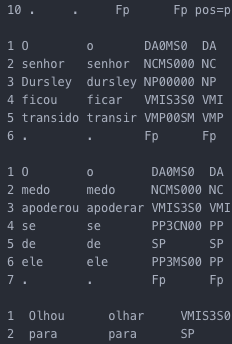
\includegraphics[scale=0.6]{analise1.png}
\caption{Exemplo de dois extratos no ficheiro harrypotter1.}
\label{img:analise1}
\end{figure}

\subsection{Personagens do Harry Potter}
\label{subsec:analise2}

///////////////////////// POR FAZER /////////////////////

Nesta segunda alínea do exercício, era requerido um filtro que criasse uma lista de provérbios (citações contidas em páginas cujo título começa por "Provérbios").

Procedendo à análise do ficheiro \textit{XML} foi possível entender a forma como se organiza a informação nas páginas que referem provérbios:


Neste caso, está exemplificada a página na qual o título é \textbf{Provérbios cipriotas}, visto que este se encontra entre as marcas \underline{<title>} e \underline{</title>}. É, portanto, desta forma que são identificadas as páginas que temos interesse em aceder. Tal facto aparece sublinhado a vermelho na figura.

Aquando da análise do ficheiro foram encontrados casos em que o título continha a palavra "Provérbio", mas não era inicializado por esta. É importante, de facto, ter em conta este caso pois tal é requirido no enunciado do exercício.

Filtrando os títulos das páginas, procuramos saber quais as marcas que indicam o início de um provérbio. Neste caso, sublinhado a verde, é possível concluir que a marca de início é \underline{* '''\&quot;} , enquanto a marca de fim é \underline{\&quot;'''}.

Realizada a análise das páginas de provérbios, foi possível concluir que existem inúmeras formas de identificar o início e o fim dum provérbio. Tal acontece porque o ficheiro contém muita variedade de idiomas e, consequentemente, diferentes ideias das diferentes pessoas que decidem quais as marcas a usar nas citações.

	\vspace{0.2cm}

Alguns exemplos de marcas de início de provérbios presentes no ficheiro são:
\begin{itemize}
 \item *\&quot;
 \item *\&quot;''
 \item **''\&quot;
 \item :'''
\end{itemize}

	\vspace{0.2cm}

Por outro lado, alguns exemplos de marcas de final de provérbios presentes no ficheiro são:
\begin{itemize}
 \item \&quot;
 \item \&quot;''
 \item ''\&quot;
 \item '''
\end{itemize}

	\vspace{0.2cm}

A ideia inicial foi generalizar as expressões regulares para qualquer página de provérbios, mas devido ao facto de existirem inúmeras marcas diversificadas foi necessário criar alguns contextos específicos para cada país, de forma a que não houvessem conflitos entre marcas e fosse possível criar um output perceptível.

Nos capítulos seguintes serão abordados pormenorizadamente estes casos.


\subsection{Palavras por Classes em HTML}

A terceira alínea do exercício requeria que fosse criado um filtro capaz de calcular uma lista de verbos, substantivos, adjectivos e advérbios. Consequentemente deveria ser colocado num ficheiro HTML cada uma destas listas.

Numa primeira abordagem ao problema foram analisadas as possíveis formas de apresentação de cada classe de palavras a serem filtradas.

Atendendo ao formato Freeling dum ficheiro CORPORA, foram de fácil verificação os seguintes factos, relativos à 6ª coluna de cada extrato:

\begin{enumerate}
 \item Se uma palavra for um verbo, então "pos=verb" está contido neste campo;
 \item Se uma palavra for um substantivo, então "pos=noun" está contido neste campo;
 \item Se uma palavra for um adjetivo, então "pos=adjective" está contido neste campo;
 \item Se uma palavra for um advérbio, então "pos=adverb" está contido neste campo;
\end{enumerate}

Foram ainda necessárias criar algumas bases na linguagem de programação HTML relativas à estruturação dum ficheiro, à criação dum cabeçalho e à listagens de elementos. Estas foram basicamente todas as operações necessárias, usadas nesta linguagem, para a realização desta alínea.


\subsection{Dicionário}

Nesta quarta alínea do exercício era requerida a apresentação de um dicionário implícito num ficheiro corpora. Este dicionário deve conter as lemas, as palavras derivadas das lemas, e a informação relativa a essas mesmas palavras. Esta informação vem dividida em colunas.

Realizando a análise de cada ficheiro concluímos que, para a resolução deste exercício o que nos interessava era:

\begin{itemize}
 \item Segunda coluna $\Rightarrow$ Palavra
 \item Terceira coluna $\Rightarrow$ Lema da Palavra
 \item Sexta coluna $\Rightarrow$ Informação da Palavra
\end{itemize}

\vspace{0.5cm}

Na figura \ref{img:analise4} é possivel verificar:

\begin{enumerate}
	\item Palavra $\Rightarrow$ Dumbledore ; Lema $\Rightarrow$ dumbledore ; Informação $\Rightarrow$ Noun Proper ;
	\item Palavra $\Rightarrow$ voltou ; Lema $\Rightarrow$ voltar ; Informação $\Rightarrow$ Verb Main Indicative Past 3 Singular ;
	\item Palavra $\Rightarrow$ se ; Lema $\Rightarrow$ se ; Informação $\Rightarrow$ Pronoun Personal 3 Common Invariable ;
	\item Palavra $\Rightarrow$ e ; Lema $\Rightarrow$ e ; Informação $\Rightarrow$ Conjunction Coordinating ;
	\item Palavra $\Rightarrow$ desceu ; Lema $\Rightarrow$ descer ; Informação $\Rightarrow$ Verb Main Indicative Past 3 Singular ;
	\item Palavra $\Rightarrow$ a ; Lema $\Rightarrow$ o ; Informação $\Rightarrow$ Determiner Article Feminine Singular ;
	\item Palavra $\Rightarrow$ rua ; Lema $\Rightarrow$ rua ; Informação $\Rightarrow$ Noun Common Feminine Singular ;
	\item Palavra $\Rightarrow$ . ; Lema $\Rightarrow$ . ; Informação $\Rightarrow$ Punctuation Period ;
\end{enumerate}


\begin{figure}[H]
\centering
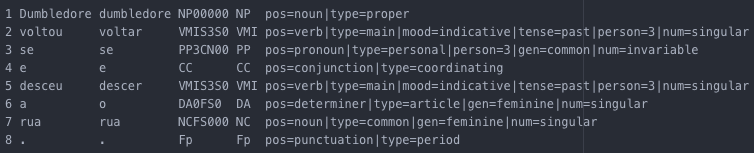
\includegraphics[scale=0.6]{analise4.png}
\caption{Exemplo de um extrato no ficheiro harrypotter1.}
\label{img:analise4}
\end{figure}


\chapter{Conceção/desenho da Resolução}
\label{chap:concecao}

///////////////////////// POR FAZER /////////////////////

Neste capítulo baseando-nos nas análises feitas ao ficheiro \emph{XML}, construímos 3 autómatos que achamos que seriam necessários para a implementação de cada um dos 3 filtros.

Os autómatos criados são uma representação de alto nível dos algoritmos implementados e serviram para criar uma base para a fase de implementação e ter uma boa noção dos contextos a utilizar. Não têm por isso, todo o detalhe que deviam uma vez que existem casos muito peculiares de implementação que não devem devem nem podem (por motivos de espaço e compreensão) ser colocados nos autómatos.

\section{Algoritmos}
\subsection{Número de Extratos}

///////////////////////// POR FAZER /////////////////////

\begin{center}
\begin{tikzpicture}[scale=0.2]
\tikzstyle{every node}+=[inner sep=0pt]
\draw [black] (9.2,-21.5) circle (3);
\draw (9.2,-21.5) node {$INITIAL$};
\draw [black] (31.7,-21.5) circle (3);
\draw (31.7,-21.5) node {$PAGE$};
\draw [black] (50.8,-21.5) circle (3);
\draw (50.8,-21.5) node {$AUTOR$};
\draw [black] (71.9,-21.5) circle (3);
\draw (71.9,-21.5) node {$QUOTE$};
\draw [black] (50.1,-39.8) circle (3);
\draw (50.1,-39.8) node {$NOME\_AUTOR$};
\draw [black] (1.6,-21.5) -- (6.2,-21.5);
\fill [black] (6.2,-21.5) -- (5.4,-21) -- (5.4,-22);
\draw [black] (28.805,-22.285) arc (-77.1203:-102.8797:37.484);
\fill [black] (28.81,-22.28) -- (27.91,-21.98) -- (28.14,-22.95);
\draw (20.45,-23.73) node [below] {$nova\_pagina$};
\draw [black] (34.7,-21.5) -- (47.8,-21.5);
\fill [black] (47.8,-21.5) -- (47,-21) -- (47,-22);
\draw (41.25,-22) node [below] {$inicio\_autor$};
\draw [black] (48.57,-37.226) arc (-155.15368:-209.22747:14.613);
\fill [black] (48.57,-37.23) -- (48.69,-36.29) -- (47.78,-36.71);
\draw (46.67,-30.51) node [left] {$nome\_autor$};
\draw [black] (52.324,-24.078) arc (24.73681:-29.11795:14.66);
\fill [black] (52.32,-24.08) -- (52.21,-25.01) -- (53.11,-24.6);
\draw (54.22,-30.79) node [right] {$nome\mbox{ }>\mbox{ }1$};
\draw [black] (47.272,-40.784) arc (-77.04436:-192.6434:13.785);
\fill [black] (30.73,-24.33) -- (30.07,-25) -- (31.04,-25.22);
\draw (29.84,-37.6) node [below] {$nome\mbox{ }=\mbox{ }"\ "$};
\draw [black] (68.978,-22.175) arc (-79.12516:-100.87484:40.429);
\fill [black] (68.98,-22.17) -- (68.1,-21.83) -- (68.29,-22.82);
\draw (61.35,-23.4) node [below] {$\*quote\_token$};
\draw [black] (53.54,-20.284) arc (110.13881:69.86119:22.683);
\fill [black] (53.54,-20.28) -- (54.46,-20.48) -- (54.12,-19.54);
\draw (61.35,-18.4) node [above] {$fim\_quote$};
\draw [black] (7.59,-18.983) arc (240.34019:-47.65981:2.25);
\draw (7.32,-13.86) node [above] {$fim\_pagina$};
\fill [black] (10.22,-18.69) -- (11.05,-18.24) -- (10.18,-17.75);
\draw [black] (12.075,-20.647) arc (104.02759:75.97241:34.551);
\fill [black] (12.08,-20.65) -- (12.97,-20.94) -- (12.73,-19.97);
\draw (20.45,-19.12) node [above] {$fim\_pagina$};
\draw [black] (11.541,-19.626) arc (125.94601:54.05399:31.445);
\fill [black] (11.54,-19.63) -- (12.48,-19.56) -- (11.9,-18.75);
\draw (30,-13.14) node [above] {$fim\_pagina$};
\draw [black] (10.875,-19.012) arc (143.70718:36.29282:36.817);
\fill [black] (10.88,-19.01) -- (11.75,-18.66) -- (10.95,-18.07);
\draw (40.55,-3.49) node [above] {$fim\_pagina$};
\end{tikzpicture}
\end{center}

\underline{Nota:}
\begin{itemize}
	\item O \emph{fim\_quote} no nosso filtro é representado em muitos casos, decidimos colocar tudo como sendo \emph{fim\_quote}.
\end{itemize}

	\vspace{1.5cm}

\textbf{Definições:}
\begin{itemize}
	\item espacos $\Rightarrow$ [\ ]*
	\item nova\_pag $\Rightarrow$ <page>
	\item fim\_pag $\Rightarrow$ </page>
	\item nome\_linguas $\Rightarrow$ (Nome|Nombre|Name)
	\item inicio\_autor $\Rightarrow$ \{\{(?i:Autor)
	\item fim\_autor $\Rightarrow$ \}\}
	\item nome\_autor $\Rightarrow$ |\{espacos\}\{nome\_linguas\}\{espacos\}=\{espacos\}
	\item quote\_token $\Rightarrow$ \{espacos\}\&quot;
\end{itemize}

\vspace{0.5cm}

\textbf{Definição do autómato:}

\begin{itemize}
	\item Estados do autómato:
		\begin{itemize}
			\item INITIAL
			\item PAGE
			\item AUTOR
			\item NOME\_AUTOR
			\item QUOTE
		\end{itemize}
	\item Estado inicial:
		\begin{itemize}
			\item INITIAL
		\end{itemize}
	\item Estados finais:
		\begin{itemize}
			\item INITIAL
			\item PAGE
			\item AUTOR
			\item NOME\_AUTOR
			\item QUOTE
		\end{itemize}
	\item Funções de Transição:
		\begin{itemize}
			\item INITIAL $\rightarrow$ $\{nova\_pagina\}$ $\rightarrow$ PAGE
			\item PAGE $\rightarrow$ $\{inicio\_autor\}$ $\rightarrow$ AUTOR
			\item PAGE $\rightarrow$ $\{fim\_pagina\} $ $\rightarrow$ INITIAL
			\item AUTOR $\rightarrow$ $\{nome\_autor\}$ $\rightarrow$ NOME\_AUTOR
			\item AUTOR $\rightarrow$ $*\{quote\_token\}$ $\rightarrow$ QUOTE
			\item AUTOR $\rightarrow$ $\{fim\_pagina\} $ $\rightarrow$ INITIAL
			\item NOME\_AUTOR $\rightarrow$ $ [ \wedge \setminus n]+\setminus n $ $\rightarrow$ PAGE ou AUTOR
			\item NOME\_AUTOR $\rightarrow$ $ [ \wedge \setminus |]+\setminus | $ $\rightarrow$ PAGE ou AUTOR
			\item NOME\_AUTOR $\rightarrow$ $\{fim\_pagina\} $ $\rightarrow$ INITIAL
			\item QUOTE $\rightarrow$ $\{fim\_quote\} $ $\rightarrow$ AUTOR
			\item QUOTE $\rightarrow$ $\{fim\_pagina\} $ $\rightarrow$ INITIAL
		\end{itemize}
\end{itemize}

\vspace{0.5cm}

\underline{Nota:}
\begin{itemize}
	\item De referir que os estados terminais deste autómato podem ser qualquer um, uma vez que que um estado final é atingido quando um filtro atinge EOF (end-of-file).
\end{itemize}



\subsection{Personagens do Harry Potter}
\label{sub:algoritmos2}

///////////////////////// POR FAZER /////////////////////

\begin{center}
\begin{tikzpicture}[scale=0.2]
\tikzstyle{every node}+=[inner sep=0pt]
\draw [black] (9.9,-32.9) circle (3);
\draw (9.9,-32.9) node {$INIT$};
\draw [black] (26.9,-32.9) circle (3);
\draw (26.9,-32.9) node {$PAGE$};
\draw [black] (57.8,-32.9) circle (3);
\draw (57.8,-32.9) node {$PC$};
\draw [black] (75.3,-32.9) circle (3);
\draw (75.3,-32.9) node {$Q$};
\draw [black] (12.9,-32.9) -- (23.9,-32.9);
\fill [black] (23.9,-32.9) -- (23.1,-32.4) -- (23.1,-33.4);
\draw (18.4,-33.4) node [below] {$nova\_pag$};
\draw [black] (12.016,-30.787) arc (126.88455:53.11545:10.637);
\fill [black] (12.02,-30.79) -- (12.96,-30.71) -- (12.36,-29.91);
\draw (18.4,-28.16) node [above] {$fim\_pag$};
\draw [black] (29.9,-32.9) -- (54.8,-32.9);
\fill [black] (54.8,-32.9) -- (54,-32.4) -- (54,-33.4);
\draw (42.35,-32.4) node [above] {$ini\_tit$Proverbios.*$fim\_tit$};
\draw [black] (72.378,-33.574) arc (-79.65641:-100.34359:32.458);
\fill [black] (72.38,-33.57) -- (71.5,-33.23) -- (71.68,-34.21);
\draw (66.55,-34.6) node [below] {$inicio\_quote$};
\draw [black] (60.641,-31.942) arc (104.90535:75.09465:22.974);
\fill [black] (60.64,-31.94) -- (61.54,-32.22) -- (61.28,-31.25);
\draw (66.55,-30.67) node [above] {$fim\_quote$};
\draw [black] (2.1,-32.9) -- (6.9,-32.9);
\fill [black] (6.9,-32.9) -- (6.1,-32.4) -- (6.1,-33.4);
\draw [black] (11.519,-30.375) arc (145.07326:34.92674:37.91);
\fill [black] (11.52,-30.37) -- (12.39,-30.01) -- (11.57,-29.43);
\draw (42.6,-13.67) node [above] {$fim\_pag$};
\draw [black] (11.598,-30.429) arc (142.43928:37.56072:28.07);
\fill [black] (11.6,-30.43) -- (12.48,-30.1) -- (11.69,-29.49);
\draw (33.85,-18.97) node [above] {$fim\_pag$};
\end{tikzpicture}
\end{center}

	\vspace{0.5cm}

\underline{Notas:}
\begin{itemize}
	\item O autômato aqui representado apenas apresenta a generalização de todos os casos particulares desenvolvidos para a resolução do enunciado do exercício.
	\item Devido a questões de perceptibilidade, as condições \textit{inicio\_quote} e \textit{fim\_quote} na representação deste autômato não são funções de transição, mas meramente indicam que nestas ações ocorrem o início e o fim de uma citação, respetivamente.
\end{itemize}

\textbf{Definições: }
\begin{itemize}
	\item espaco $\Rightarrow$ (\ )
	\item espacos $\Rightarrow$ [\ ]*
	\item nova\_pag $\Rightarrow$ <page>
	\item fim\_pag $\Rightarrow$ </page>
	\item ini\_tit $\Rightarrow$ <title>
	\item fim\_tit $\Rightarrow$ </title>
	\item quote\_token $\Rightarrow$ \{espacos\}\&quot;\{espacos\}
	\item letras $\Rightarrow$ [A-Za-z]+
	\item especiais $\Rightarrow$ [
\end{itemize}

	\vspace{0.5cm}

\textbf{Definição do autómato:}

\begin{itemize}
	\item Estados do autómato:
		\begin{itemize}
			\item INIT $\Rightarrow$ INITIAL
			\item PAGE
			\item PC $\Rightarrow$ PAGE\_CONTEUDO
			\item Q $\Rightarrow$ QUOTE
		\end{itemize}
	\item Estado inicial: INIT
	\item Estados finais:
		\begin{itemize}
			\item INIT $\Rightarrow$ INITIAL
			\item PAGE
			\item PC $\Rightarrow$ PAGE\_CONTEUDO
			\item Q $\Rightarrow$ QUOTE
		\end{itemize}
	\item Funções de Transição:
		\begin{itemize}
			\item INITIAL $\rightarrow$ $\{nova\_pag\}$ $\rightarrow$ PAGE
			\item PAGE $\rightarrow$ $\{ini\_tit\}$Proverbios.*$\{fim\_tit\}$ $\rightarrow$ PAGE\_CONTEUDO
			\item PAGE\_CONTEUDO $\rightarrow$ $inicio\_quote$ $\rightarrow$ QUOTE
			\item QUOTE $\rightarrow$ .* $fim\_quote$ $\rightarrow$ PAGE\_CONTEUDO
			\item * $\rightarrow$ $\{fim\_pag\}$ $\rightarrow$ INITIAL
		\end{itemize}
\end{itemize}

\vspace{0.5cm}

\underline{Nota:}
\begin{itemize}
	\item De referir que os estados terminais deste autómato podem ser qualquer um, uma vez que que um estado final é atingido quando um filtro atinge EOF (end-of-file).
\end{itemize}



\newpage

\subsection{Palavras por Classes em HTML}
\label{sub:algoritmos3}

///////////////////////// POR FAZER /////////////////////

\begin{center}
\begin{tikzpicture}[scale=0.2]
\tikzstyle{every node}+=[inner sep=0pt]
\draw [black] (8.9,-4.7) circle (3);
\draw (8.9,-4.7) node {$INIT$};
\draw [black] (25.8,-4.7) circle (3);
\draw (25.8,-4.7) node {$PAGE$};
\draw [black] (57.8,-4.7) circle (3);
\draw (57.8,-4.7) node {$PC$};
\draw [black] (40.4,-18.5) circle (3);
\draw (40.4,-18.5) node {$Q$};
\draw [black] (40.4,-29.9) circle (3);
\draw (40.4,-29.9) node {$QC$};
\draw [black] (17.1,-38.6) circle (3);
\draw (17.1,-38.6) node {$ADU$};
\draw [black] (63.3,-38.6) circle (3);
\draw (63.3,-38.6) node {$ALT$};
\draw [black] (17.1,-56.4) circle (3);
\draw (17.1,-56.4) node {$QADU$};
\draw [black] (63.3,-56.4) circle (3);
\draw (63.3,-56.4) node {$QALT$};
\draw [black] (10.223,-7.38) arc (54:-234:2.25);
\draw (8.9,-11.95) node [below] {$fim\_pag$};
\fill [black] (7.58,-7.38) -- (6.7,-7.73) -- (7.51,-8.32);
\draw [black] (11.9,-4.7) -- (22.8,-4.7);
\fill [black] (22.8,-4.7) -- (22,-4.2) -- (22,-5.2);
\draw (17.35,-5.2) node [below] {$nova\_pag$};
\draw [black] (2.1,-4.7) -- (5.9,-4.7);
\fill [black] (5.9,-4.7) -- (5.1,-4.2) -- (5.1,-5.2);
\draw [black] (28.8,-4.7) -- (54.8,-4.7);
\fill [black] (54.8,-4.7) -- (54,-4.2) -- (54,-5.2);
\draw (41.8,-5.2) node [below] {$ini\_tit$Proverbios.*$fim\_tit$};
\draw [black] (55.45,-6.56) -- (42.75,-16.64);
\fill [black] (42.75,-16.64) -- (43.69,-16.53) -- (43.07,-15.75);
\draw (55.33,-12.1) node [below] {$*quote\_token$};
\draw [black] (39.563,-27.024) arc (-169.37552:-190.62448:15.318);
\fill [black] (39.56,-27.02) -- (39.91,-26.15) -- (38.92,-26.33);
\draw (38.8,-24.2) node [left] {.*$quote\_token$};
\draw [black] (37.697,-31.201) arc (-65.0152:-74.03449:120.165);
\fill [black] (19.99,-37.81) -- (20.9,-38.07) -- (20.63,-37.11);
\draw (35.41,-35.52) node [below] {$**adulterados$};
\draw [black] (43.398,-29.835) arc (88.28203:50.11313:28.961);
\fill [black] (61.1,-36.56) -- (60.81,-35.66) -- (60.17,-36.43);
\draw (59.34,-31.05) node [above] {$**alternativos$};
\draw [black] (19.719,-37.137) arc (118.00528:102.94504:72.268);
\fill [black] (19.72,-37.14) -- (20.66,-37.2) -- (20.19,-36.32);
\draw (21.94,-32.57) node [above] {$**adulteracao$};
\draw [black] (17.156,-35.604) arc (-185.50339:-272.93049:19.371);
\fill [black] (37.43,-18.12) -- (36.65,-17.58) -- (36.6,-18.57);
\draw (17.55,-22.3) node [above] {$*quote\_token$};
\draw [black] (16.426,-53.478) arc (-169.60117:-190.39883:33.118);
\fill [black] (16.43,-53.48) -- (16.77,-52.6) -- (15.79,-52.78);
\draw (15.38,-47.5) node [left] {$***quote\_token$};
\draw [black] (62.681,-53.466) arc (-170.46728:-189.53272:36.021);
\fill [black] (62.68,-53.47) -- (63.04,-52.59) -- (62.06,-52.76);
\draw (61.68,-47.5) node [left] {$***quote\_token$};
\draw [black] (43.381,-18.188) arc (91.55223:5.89903:19.419);
\fill [black] (43.38,-18.19) -- (44.19,-18.67) -- (44.17,-17.67);
\draw (62.95,-22.52) node [above] {$*quote\_token$};
\draw [black] (60.305,-38.77) arc (-86.97892:-93.02108:381.471);
\fill [black] (20.1,-38.77) -- (20.87,-39.31) -- (20.92,-38.31);
\draw (40.2,-39.8) node [below] {$**adulterados$};
\draw [black] (60.532,-39.755) arc (-68.8716:-111.1284:56.405);
\fill [black] (19.87,-39.76) -- (20.43,-40.51) -- (20.79,-39.58);
\draw (40.2,-44.05) node [below] {$**adulteracao$};
\draw [black] (17.873,-41.497) arc (11.97339:-11.97339:28.935);
\fill [black] (17.87,-41.5) -- (17.55,-42.38) -- (18.53,-42.18);
\draw (19,-47.5) node [right] {.*$quote\_token$};
\draw [black] (64.243,-41.446) arc (14.72619:-14.72619:23.817);
\fill [black] (64.24,-41.45) -- (63.96,-42.35) -- (64.93,-42.09);
\draw (65.53,-47.5) node [right] {.*$quote\_token$};
\draw [black] (41.089,-21.416) arc (8.65405:-8.65405:18.5);
\fill [black] (41.09,-21.42) -- (40.72,-22.28) -- (41.7,-22.13);
\draw (41.8,-24.2) node [right] {$*quote\_token$};
\end{tikzpicture}
\end{center}

\underline{Nota:}
\begin{itemize}
	\item Todos os estados do autômato possuem uma condição \textit{fim\_pag} para o estado INIT. Neste autômato só está representado no próprio estado INIT.
\end{itemize}

	\vspace{1.0cm}

\textbf{Definições: }
\begin{itemize}
	\item espacos $\Rightarrow$ [\ ]*
	\item nova\_pag $\Rightarrow$ <page>
	\item fim\_pag $\Rightarrow$ </page>
	\item ini\_tit $\Rightarrow$ <title>
	\item fim\_tit $\Rightarrow$ </title>
	\item quote\_token $\Rightarrow$ \{espacos\}\&quot;
	\item adulteracao $\Rightarrow$ \{espacos\}'''Adulteração:'''
	\item alternativos $\Rightarrow$ \{espacos\}'''Alternativos:'''
	\item adulterados $\Rightarrow$ \{espacos\}'''Adulterados:'''
\end{itemize}

	\vspace{1.0cm}

\textbf{Definição do autómato:}

\begin{itemize}
	\item Estados do autómato:
		\begin{itemize}
			\item INIT $\Rightarrow$ INITIAL
			\item PAGE
			\item PC $\Rightarrow$ PAGE\_CONTEUDO
			\item Q $\Rightarrow$ QUOTE
			\item QC $\Rightarrow$ QUOTE\_CONT
			\item ADU $\Rightarrow$ ADULTERADOS
			\item ALT $\Rightarrow$ ALTERNATIVOS
			\item QADU $\Rightarrow$ QUOTES\_ADULTERADOS
			\item QALT $\Rightarrow$ QUOTES\_ALTERNATIVOS
		\end{itemize}
	\item Estado inicial: INIT
	\item Estados finais:
		\begin{itemize}
			\item INIT $\Rightarrow$ INITIAL
			\item PAGE
			\item PC $\Rightarrow$ PAGE\_CONTEUDO
			\item Q $\Rightarrow$ QUOTE
			\item QC $\Rightarrow$ QUOTE\_CONT
			\item ADU $\Rightarrow$ ADULTERADOS
			\item ALT $\Rightarrow$ ALTERNATIVOS
			\item QADU $\Rightarrow$ QUOTES\_ADULTERADOS
			\item QALT $\Rightarrow$ QUOTES\_ALTERNATIVOS
		\end{itemize}
	\item Funções de Transição:
		\begin{itemize}
			\item INITIAL $\rightarrow$ $\{nova\_pag\}$ $\rightarrow$ PAGE
			\item PAGE $\rightarrow$ $\{ini\_tit\}$Proverbios.*$\{fim\_tit\}$ $\rightarrow$ PAGE\_CONTEUDO
			\item PAGE\_CONTEUDO $\rightarrow$ $*\{quote\_token\}$ $\rightarrow$ QUOTE
			\item QUOTE $\rightarrow$ .* $*\{quote\_token\}$ $\rightarrow$	QUOTE\_CONT
			\item QUOTE\_CONT $\rightarrow$ $*\{quote\_token\}$ $\rightarrow$ QUOTE
			\item QUOTE\_CONT $\rightarrow$ $**\{adulterados\}$ $\rightarrow$ ADULTERADOS
			\item QUOTE\_CONT $\rightarrow$ $**\{adulteracao\}$ $\rightarrow$ ADULTERADOS
			\item QUOTE\_CONT $\rightarrow$ $**\{alternativos\}$ $\rightarrow$ ALTERNATIVOS
			\item ADULTERADOS $\rightarrow$ $***\{quote\_token\}$ $\rightarrow$ QUOTES\_ADULTERADOS
			\item ADULTERADOS $\rightarrow$ $*\{quote\_token\}$ $\rightarrow$ QUOTE
			\item ALTERNATIVOS $\rightarrow$ $***\{quote\_token\}$ $\rightarrow$ QUOTES\_ALTERNATIVOS
			\item ALTERNATIVOS $\rightarrow$ $*\{quote\_token\}$ $\rightarrow$ QUOTE
			\item ALTERNATIVOS $\rightarrow$ $**\{adulterados\}$ $\rightarrow$ ADULTERADOS
			\item ALTERNATIVOS $\rightarrow$ $**\{adulteracao\}$ $\rightarrow$ ADULTERADOS
			\item QUOTES\_ADULTERADOS $\rightarrow$ .* $*\{quote\_token\}$ $\rightarrow$ ADULTERADOS
			\item QUOTES\_ALTERNATIVOS $\rightarrow$ .* $*\{quote\_token\}$ $\rightarrow$ ALTERNATIVOS
			\item * $\rightarrow$ $\{fim\_pag\}$ $\rightarrow$ INITIAL
		\end{itemize}
\end{itemize}

\vspace{0.5cm}

\underline{Nota:}
\begin{itemize}
	\item De referir que os estados terminais deste autómato podem ser qualquer um, uma vez que que um estado final é atingido quando um filtro atinge EOF (end-of-file).
\end{itemize}

\subsection{Dicionário}
\label{sub:algoritmos4}

///////////////////////// POR FAZER /////////////////////


\chapter{Codificação e Testes}
\label{chap:codificacao}

///////////////////////// POR FAZER /////////////////////

Para a presente secção de codificação e testes baseámo-nos nos capítulos anteriores, pois ambos são extremamente importantes para uma boa implementação desta fase. O capítulo de análise teve a sua relevância pois permitiu-nos ter já uma ideia de que expressões regulares utilizar para filtrar o que desejávamos e o capítulo da conceção da resolução foi relevante pois definimos os autómatos necessários e os contextos precisos para coordenar o processo de filtragem para cada requisito.

\section{Estruturas de Dados}
\subsection{?????????}

///////////////////////// POR FAZER /////////////////////

Quando começamos a desenvolver os primeiros filtros para testar com o ficheiro de input, deparamo-nos com a situação de existir mais que uma página para um mesmo autor. Seria portanto ideal que armazenássemos todas as citações referentes a um autor numa \textbf{Tabela de Hash} e íamos inserindo a esta as citações que aparecessem em diferentes páginas referentes a um mesmo autor.

Adotanto esta abordagem temos que filtrar tudo o que é necessário e só no fim despejar para o ecrã, de forma organizada, tudo aquilo que armazenamos na estrutura.

Desta forma criamos uma estrutura \textbf{TodasCitações}, que contém uma \textbf{GHashTable} cuja chave é o nome do autor e o valor é uma outra estrutura \textbf{Autor} que contém um nome e uma lista de citações. Estas estruturas são apresentadas nas seguintes imagens.


\section{Alternativas, Decisões e Problemas de Implementação}

\subsection{Número de Extratos}

///////////////////////// POR FAZER /////////////////////

Ao implementar esta questão começou-se por reparar que nem todas as páginas de autor estão de facto identificadas por um autor. Desta forma foi necessário ignorar todas as páginas de autor que não fossem identificadas por um autor que tivesse um nome com tamanho superior a 1.

O maior problema neste filtro foi identificar todas as formas como uma citação acabava e gerir esta questão. Encontrámos ao todo 10 formas diferentes de término duma citação e alguns dos casos são muito parecidos, de facto são especializações de casos mais gerais, pelo que a tarefa de encontrar o término duma citação ficou dificultada.

A propriedade \emph{longest match} do \textbf{flex}, foi outro entrave à implementação uma vez que como tínhamos casos que eram especialização de outros, muitas vezes o caso que era o \emph{longest match} não era o que era pretendido que fosse apanhado. Esta é a razão pela qual aparecem \textbf{\&quot;} no final de algumas citações.

Muita vezes fomo-nos deparando com citações que continham \textbf{\&quot;} não no final mas sim no meio das citações. Decidimos considerar que estes "tokens"  fariam parte da citação uma vez que apanhámos a citação toda até uma situação de término, ignorando o conteúdo de cada citação.

Para a realização deste filtro utilizámos as estruturas descritas acima em conjunto com algumas funções auxiliares que no permitiam inserir citações, autores, e ainda imprimir todas as citações da estrutura existente.


\subsection{Personagens do Harry Potter}

///////////////////////// POR FAZER /////////////////////

Tendo em conta a grande variedade de marcas para representar provérbios em diferentes países, a resolução desta questão foi condicionada por tal. Desta forma, são muitos os estados criados para as mesmas partes de diferentes páginas do ficheiro.

Após a análise explicada na secção \ref{subsec:analise2} foi possível concluir quais seriam os casos mais críticos. São exemplo disso os provérbios russos, que têm como marca inicial apenas \underline{*}. Devido à elevada ocorrência desta marca em todo o ficheiro, foi necessário limitar a filtragem com esta marca apenas à parte do ficheiro que pretendiamos, e tal foi possível através do conceito de Estado.

Relembrando o autómato apresentado na secção \ref{sub:algoritmos2}, existem quatro fases importantes no algoritmo.

Na fase inicial vamos percorrer as páginas do ficheiro. Na segunda fase vamos interpretar o título da página e, tendo em conta o resultado obtido, o estado seguinte vai ser diferente. Existe o caso \textit{default} que apanha tudo o que aparece em frente à palavra \textit{Provérbios} mas, devido à grande variedade de marcas, tivemos aqui que forçar alguns processos a seguir caminhos particulares, sendo nesses casos a condição o título inteiro, como por exemplo \textit{Provérbios russos}.

A partir deste momento o estado passa a seguir um caminho particular, que é o \textit{CONTEUDO\_RUS}. Esta é, portanto, a terceira fase. Depois de estar no conteúdo russo e serem atingidas as marcas de início de provérbio, o estado passa a ser o \textit{QUOTE\_RUS}, que vai ler a citação e, de seguida, imprimi-la no ecrã com a formatação desejada. Esta quarta fase regressa depois ao conteúdo da página de provérbios russos para continuar a sua filtragem.

Após a análise total das páginas, e de forma a não ter contextos em exagero, tentamos unificar num só contexto os países que teriam as mesmas marcas, ou marcas que fossem compatíveis. São exemplos deste facto os provérbios turcos, búlgaros, chineses e holandeses, que são compatíveis e deram origem aos estados CONTEUDO\_TURQ\_BUL\_CHI\_HOL e QUOTE\_TURQ\_BUL\_CHI\_HOL.


\newpage

\subsection{Palavras por Classes em HTML}

///////////////////////// POR FAZER /////////////////////

A abordagem a esta questão é diferente das anteriores. Ao invês de possuir muitos casos particulares, a resolução desta questão possui antes um maior encadeamento de estados, como foi possível concluir na secção \ref{sub:algoritmos3}. Tal acontece porque estamos interessados em saber provérbios que estejam relacionados com outros provérbios.

A fase inicial de filtrar os títulos funciona tal e qual como na questão 2. Depois de estar no conteúdo duma página, o algoritmo é diferente.

Primeiro lemos o provérbio e guardamo-lo em memória, fazendo uso da função \textit{strdup}. Se a linha seguinte for uma das marcas que indicam que vão ser listados os provérbios alternativos ou adulterados, imprimi-mos no ecrã o provérbio que tinha sido guardado. Caso contrário, continuamos a filtragem normalmente.

Caso a marca atingível seja a dos provérbios adulterados, vai ser iniciada na linha seguinte a listagem destes mesmos. Estes provérbios vão ser impressos e marcados como adulterados no output do filtro. A listagem termina quando a marca deixar de ser \underline{***}.

Tal processo acontece também com os provérbios alternativos, sendo que estes têm apenas uma diferença nos estados ao qual se dirigem. Após análise do ficheiro foi possível concluir que os provérbios adulterados, caso existam, sucedem sempre os provérbios alternativos. Desta forma é necessário, depois de listar os provérbios alternativos, verificar também os adulterados do provérbio original, caso surja a marca destes.


\subsection{Dicionário}

///////////////////////// POR FAZER /////////////////////


\section{Testes realizados e Resultados}
\subsection{Número de Extratos}

///////////////////////// POR FAZER /////////////////////

Aplicando o filtro criado para a primeira questão com o ficheiro de input disponibilizado, podem-se verificar resultados com um formato muito parecido ao da seguinte imagem.

Foram apenas imprimidas citações de autores que existam e no final é apresentada uma estatística da filtragem, que contempla o número de páginas total, o número de páginas de autor, o número de autores e o número de citações.


\subsection{Lista de Provérbios}

///////////////////////// POR FAZER /////////////////////

Tendo em conta a imensa variedade de marcas de início de provérbios, nesta fase os testes tiveram uma enorme importância.

O resultado do filtro está organizado por Título e Citações, sendo que no final é apresentada uma estatística da filtragem, que contempla o número de páginas total, o número de páginas com título começado por 'Provérbios', e o número de citações recolhidas no filtro.

Seguem-se alguns exemplos de provérbios obtidos da filtragem.


\newpage

\subsection{Palavras por Classes em HTML}

///////////////////////// POR FAZER /////////////////////

O resultado do filtro está organizado por Título e Citações (com os seus adulterados), sendo que no final é apresentada uma estatística da filtragem, que contempla o número de páginas total, o número de páginas com título começado por 'Provérbios', o número de adulterações, o número de alternativos, e o número de citações recolhidas no filtro.

Seguem-se alguns exemplos de provérbios obtidos da filtragem.

\newpage

\subsection{Dicionário}


///////////////////////// POR FAZER /////////////////////

As seguintes imagens representam os resultados de cada filtro realizado, que aparecem no final de cada filtragem.



\chapter{Conclusão}
\label{chap:concl}

///////////////////////// POR FAZER /////////////////////

Tendo em conta os requisitos deste projeto, e o trabalho realizado pelo grupo, achamos que os objetivos fundamentais foram atingidos, sendo estes a capacidade de criar padrões com uso de \textbf{Expressões Regulares}, o entendimento da utilização da ferramenta \textbf{flex} para a criação destes padrões, a capacidade de analisar ficheiros de entrada e criar algoritmos de resolução recorrendo a \textbf{autómatos}.

Ao longo da realização deste projeto o grupo encontrou várias dificuldades, estando estas relacionadas maioritariamente com a quantidade de formas diferentes em que apareciam as citações e os provérbios a serem filtrados. Entendemos portanto, que esta foi a maior dificuldade pois foi necessário a agilização dos membros do grupo para encontrarem soluções para a filtragem de certos padrões.

Em jeito de conclusão o grupo acha que todas as alíneas requisitadas no enunciado foram terminadas com sucesso, e os objetivos principais deste projeto foram atingidos.


\end{document}
